\chapter{Expresiones y programas simples}
\section{Evaluación de expresiones}

Sin usar el computador, evalúe las siguientes expresiones, y para cada
una de ellas indique el resultado y su tipo (si la expresión es válida)
o qué error ocurre (si no lo es):

\begin{lstlisting}
>>> 2 + 3      # Respuesta: tipo int, valor 5
>>> 4 / 0      # Respuesta: error de division por cero
>>> 5 + 3 * 2
>>> '5' + '3' * 2
>>> 2 ** 10 == 1000 or 2 ** 7 == 100
>>> int("cuarenta")
>>> 70/16 + 100/24
>>> 200 + 19%
>>> 3 < (1024 % 10) < 6
>>> 'six' + 'eight'
>>> 'six' * 'eight'
>>> float(-int('5') + int('10'))
>>> abs(len('ocho') - len('cinco'))
>>> bool(14) or bool(-20)
>>> float(str(int('5' * 4) / 3)[2])
\end{lstlisting}

Compruebe sus respuestas en el computador.
       % :)
\section{Saludo}

Escriba un programa que pida al usuario que escriba su nombre, y lo
salude llamándolo por su nombre.

\begin{lstlisting}[language=testcase]
Ingrese su nombre: `Perico`
Hola, Perico
\end{lstlisting}
                       % :)
\section{Círculos}

Escriba un programa que reciba como entrada el radio de un círculo y
entregue como salida su perímetro y su área:

\begin{lstlisting}[language=testcase]
Ingrese el radio: `5`
Perimetro: 31.4
Area: 78.5
\end{lstlisting}
                     % :)
\section{Promedio}

Escriba un programa que calcule el promedio de 4 notas ingresadas por el
usuario:
                     % :)
\section{Conversión de unidades de longitud}

Escriba un programa que convierta de centímetros a pulgadas. Una pulgada
es igual a 2.54 centímetros.

\begin{lstlisting}[language=testcase]
Ingrese longitud: `45`
45 cm = 17.7165 in
\end{lstlisting}


\begin{lstlisting}[language=testcase]
Ingrese longitud: `13`
13 cm = 5.1181 in
\end{lstlisting}
 % :)
\section{Número invertido}

Escriba un programa que pida al usuario un entero de tres dígitos, y
entregue el número con los dígitos en orden inverso:
             % :)
%\section{Pitágoras}

Escriba un programa que reciba como entrada las longitudes de los dos
catetos `a` y `b` de un triángulo rectángulo, y que entregue como salida
el largo de la hipotenusa `c` del triangulo, dado por el
\href{http://es.wikipedia.org/wiki/Teorema\_de\_Pit\%C3\%A1goras}{teorema
de Pitágoras}: `c\^{}2 = a\^{}2 + b\^{}2`.

\section{Hora futura}

Escriba un programa que pregunte al usuario la hora actual \emph{t} del
reloj y un número entero de horas \emph{h}, que indique qué hora marcará
el reloj dentro de \emph{h} horas:
                  % :)
\section{Parte decimal}

Escriba un programa que entregue la parte decimal de un número real
ingresado por el usuario.

\begin{lstlisting}[language=testcase]
Ingrese un numero: `4.5`
0.5
\end{lstlisting}

\begin{lstlisting}[language=testcase]
Ingrese un numero: `-1.19`
0.19
\end{lstlisting}



%\section{Qué nota necesito}

Un alumno desea saber que nota necesita en el tercer certamen para
aprobar un ramo.

El promedio del ramo se calcula con la siguiente formula.

\[N_C = \frac{(C1+C2+C3)}{3}\]\[N_F = N_C\cdot 0.7 + N_L\cdot 0.3\]

Donde `N\_C` es el promedio de certámenes, `N\_L` el promedio de
laboratorio y `N\_F` la nota final.

Escriba un programa que pregunte al usuario las notas de los dos
primeros certamen y la nota de laboratorio, y muestre la nota que
necesita el alumno para aprobar el ramo con nota final 60.

%\section{Huevos a la copa}

\emph{Ejercicio sacado de} {[}Lang09{]}\_.

Cuando un huevo es hervido en agua, las proteínas comienzan a coagularse
cuando la temperatura sobrepasa un punto crítico. A medida que la
temperatura aumenta, las reacciones se aceleran.

En la clara, las proteínas comienzan a coagularse para temperaturas
sobre 63°C, mientras que en la yema lo hacen para temperaturas sobre
70°C. Para hacer un huevo a la copa, la clara debe haber sido calentada
lo suficiente para coagularse a más de 63°C, pero la yema no debe
sobrepasar los 70°C para evitar obtener un huevo duro.

El tiempo en segundos que toma al centro de la yema alcanzar `T\_y` °C
está dado por la fórmula:

\[t = \frac{M^{2/3} c \rho^{1/3}}
{K\pi^2(4\pi/3)^{2/3}}
\ln\left[
0.76\frac{T_o - T_w}
{T_y - T_w}
\right],\]

donde `M` es la masa del huevo, `rho` su densidad, `c` su capacidad
calorífica específica y `K` su conductividad térmica. Algunos valores
típicos son:

\begin{itemize}
\item
  `M = 47,{[}text\{g\}{]}` para un huevo pequeño y `M =
  67,{[}text\{g\}{]}` para uno grande,
\item
  `rho = 1.038,{[}text\{g\},text\{cm\}\^{}\{-3\}{]}`,
\item
  `c = 3.7,{[}text\{J\},text\{g\}\^{}\{-1\} text\{K\}\^{}\{-1\}{]}`, y
\item
  `K = 5.4cdot 10\^{}\{-3\},{[}text\{W\},text\{cm\}\^{}\{-1\}
  text\{K\}\^{}\{-1\}`{]}.
\end{itemize}

`T\_w` es la temperatura de ebullición del agua y `T\_o` la temperatura
original del huevo antes de meterlo al agua, ambos en grados Celsius.

Escriba un programa que reciba como entrada la temperatura original del
huevo y muestre como salida el tiempo en segundos que le toma alcanzar
la temperatura máxima para prepararlo a la copa.


\chapter{Estructuras condicionales}
\section{Determinar par}

Escriba un programa que determine si el número entero ingresado por el
usuario es par o no.
                  % :)
\section{Años bisiestos}

Cuando la Tierra completa una órbita alrededor del Sol, no han
transcurrido exactamente 365 rotaciones sobre sí misma, sino un poco
más. Más precisamente, la diferencia es de más o menos un cuarto de día.

Para evitar que las estaciones se desfasen con el calendario, el
calendario juliano introdujo la regla de introducir un día adicional en
los años divisibles por 4 (llamados
\href{http://es.wikipedia.org/wiki/A\%C3\%B1o\_bisiesto}{bisiestos}),
para tomar en consideración los cuatro cuartos de día acumulados.

Sin embargo, bajo esta regla sigue habiendo un desfase, que es de
aproximadamente \(3/400\) de día.

Para corregir este desfase, en el año 1582 el papa Gregorio XIII
introdujo un nuevo calendario, en el que el último año de cada siglo
dejaba de ser bisiesto, a no ser que fuera divisible por 400.

Escriba un programa que indique si un año es bisiesto o no, teniendo en
cuenta cuál era el calendario vigente en ese año:

\begin{lstlisting}[language=testcase]
Ingrese un anno: `1988`
1988 es bisiesto
\end{lstlisting}

\begin{lstlisting}[language=testcase]
Ingrese un anno: `2011`
2011 no es bisiesto
\end{lstlisting}

\begin{lstlisting}[language=testcase]
Ingrese un anno: `1700`
1700 no es bisiesto
\end{lstlisting}

\begin{lstlisting}[language=testcase]
Ingrese un anno: `1500`
1500 es bisiesto
\end{lstlisting}

\begin{lstlisting}[language=testcase]
Ingrese un anno: `2400`
2400 es bisiesto
\end{lstlisting}

                    % :)
%\section{División}

Escriba un programa que pida dos números enteros y que calcule la
división, indicando si la división es exacta o no.

\section{Palabra más larga}

Escriba un programa que pida al usuario dos palabras, y que indique cuál
de ellas es la más larga y por cuántas letras lo es.

\begin{lstlisting}[language=testcase]
Palabra 1: `edificio`
Palabra 2: `tren`
La palabra edificio tiene 4 letras mas que tren.
\end{lstlisting}

\begin{lstlisting}[language=testcase]
Palabra 1: `sol`
Palabra 2: `paralelepipedo`
La palabra paralelepipedo tiene 11 letras mas que sol
\end{lstlisting}

\begin{lstlisting}[language=testcase]
Palabra 1: `plancha`
Palabra 2: `lapices`
Las dos palabras tienen el mismo largo
\end{lstlisting}


            % :)
\section{Ordenamiento}

Escriba un programa que reciba como entrada dos números, y los muestre
ordenados de menor a mayor:

\begin{lstlisting}[language=testcase]
Ingrese numero: `51`
Ingrese numero: `24`
24 51
\end{lstlisting}

A continuación, escriba otro programa que haga lo mismo con tres
números:

\begin{lstlisting}[language=testcase]
Ingrese numero: `8`
Ingrese numero: `1`
Ingrese numero: `4`
1 4 8
\end{lstlisting}

Finalmente, escriba un tercer programa que ordene cuatro números:

\begin{lstlisting}[language=testcase]
Ingrese numero: `7`
Ingrese numero: `0`
Ingrese numero: `6`
Ingrese numero: `1`
0 1 6 7
\end{lstlisting}

Recuerde que su programa debe entregar la solución correcta para
cualquier combinación de números, no sólo para los ejemplos mostrados
aquí.

Hay más de una manera de resolver cada ejercicio.
          % :)
%\section{Letra o número}

Escriba un programa que determine si un caracter ingresado es letra,
número, o ninguno de los dos. En caso que sea letra, determine si es
mayúscula o minúscula.

%\chapter{Calculadora simple}

El siguiente programa es una calculadora simple:

Al ejecutar el programa, primero uno ingresa la operación que será
aplicada, que puede ser:

\ctable[pos = H, center, botcap]{ll}
{% notes
}
{% rows
\FL
Signo & Operación
\\\noalign{\medskip}
------- & ---------------
\\\noalign{\medskip}
\lstinline!+! & Suma
\\\noalign{\medskip}
\lstinline!-! & Resta
\\\noalign{\medskip}
\lstinline!*! & Multiplicación
\\\noalign{\medskip}
\lstinline!/! & División
\\\noalign{\medskip}
\lstinline!^! & Potencia
\LL
}

La multiplicación también puede ser indicada con una \lstinline!x!
minúscula.

A continuación, se debe ingresar los dos operandos. Finalmente, el
programa muestra el resultado de la operación.

Escriba, compile y ejecute este programa.

En este programa puede ver que es posible asignar un valor inicial a una
variable al momento de declararla:

\begin{lstlisting}
float resultado = 1.0;
int valido = 1;
\end{lstlisting}

También note que tanto en el \lstinline!if! como en el \lstinline!else!
del final se ha omitido los paréntesis de llave (\lstinline!{}!) ya que
en ambos casos hay incluída solamente una única sentencia.

\section{Definición de funciones}

Al principio del programa, se ha definido una función llamada
\lstinline!potencia!. Ella recibe como parámetros la base (un número
real) y el exponente (un entero), y retorna el resultado de elevar la
base al exponente.

En C no existe un operador «elevado a» (como el \lstinline!**! de
Python), por lo que sí es útil definir una función como ésta.

Es necesario especificar explícitamente cuál será el tipo del valor
retornado (en este caso \lstinline!float!) y los tipos de cada uno de
los parámetros (en el ejemplo, \lstinline!float! e \lstinline!int!).

Las variables declaradas dentro de la función se llaman
\textbf{variables locales}. Estas variables comienzan a existir al
momento de llamar a la función, y desaparecen cuando la función termina.
Son invisibles desde fuera de la función.

En nuestro programa, las dos funciones \lstinline!main! y
\lstinline!potencia! tienen una variable local llamada
\lstinline!resultado!. Ambas variables son distintas, y sus valores
respectivos están almacenados en regiones diferentes de la memoria.

\section{Tipo char}

El tipo \lstinline!char! se usa para representar caracteres (símbolos)
solitarios. La variable \lstinline!op! que almacena la operación es de
este tipo.

Un valor de tipo \lstinline!char! se representa en un programa entre
comillas simples. Por ejemplo, el signo más está representado como
\lstinline!'+'!.

Técnicamente, los valores de tipo \lstinline!char! son números enteros
que están comprendidos entre −128 y 127. Cada número está asociado a un
caracter a través de la
\href{http://es.wikipedia.org/wiki/C\%C3\%B3digo\_ASCII\#Caracteres\_imprimibles\_ASCII}{tabla
ASCII}. Los enteros y los caracteres asociados son intercambiables; por
ejemplo, la expresión \lstinline!'m' == 109! es evaluada como verdadera.

No hay que confundir un caracter con un string de largo uno:
\lstinline!'a'! y \lstinline!"a"! son dos cosas distintas.

\section{Sentencia switch}

El \textbf{switch} es una sentencia de control condicional que permite
indicar qué hacer si el resultado de una expresión es igual a alguno de
ciertos valores constantes indicados

Un ejemplo de uso de \lstinline!switch! es el siguiente:

\begin{lstlisting}
switch (expresion) {
    case 1:
        /* que hacer cuando expresion == 1 */

    case 2:
        /* que hacer cuando expresion == 2 */

    default:
        /* que hacer cuando la expresion no es igual
         * a ninguno de los casos anteriores */
}
\end{lstlisting}

Cuando el resultado de la expresión es igual a alguno de los valores
indicados, la ejecución del programa salta al \lstinline!case! con ese
valor. Si el valor con el resultado no existe, salta a
\lstinline!default!.

Hay que tener cuidado con una característica extraña del
\lstinline!switch!: cuando se cumple un caso, los casos que vienen a
continuación también se ejecutan. En este ejemplo:

\begin{itemize}
\item
  si \lstinline!expresion == 1!, el programa saltará a
  \lstinline!case 1!, y luego continuará con \lstinline!case 2! y
  \lstinline!default!;
\item
  si \lstinline!expresion == 2!, el programa saltará a
  \lstinline!case 2!, y luego continuará con \lstinline!default!;
\item
  si \lstinline!expresion! no es ni 1 ni 2, el programa saltará a
  \lstinline!default!.
\end{itemize}

Para evitar que los casos siguientes sean ejecutados, debe ponerse un
\lstinline!break! al final de cada caso. Esto es lo que se hizo en el
programa de la calculadora.

\section{Conversión de tipos}

El segundo parámetro de la función \lstinline!potencia! es entero, pero
los operandos ingresados por el usuario son almacenados como números
reales.

Para convertir el exponente de real a entero, basta con anteponer al
valor el tipo entre paréntesis.

En este caso particular, la conversión se hace truncando los decimales
del número real. Así, si \lstinline!y! vale \lstinline!5.9!, entonces
\lstinline!(int) y! vale \lstinline!5!. Para conversiones entre otros
tipos, se siguen otras reglas diferentes.

En inglés, el nombre de esta operación es \emph{cast}. Posiblemente
usted escuche más de una vez a alguien refiriéndose a esta operación
como «castear».

\section{Ejercicios}

Modifique el programa de modo que soporte una nueva operación: obtener
el \href{http://es.wikipedia.org/wiki/Coeficiente\_binomial}{coeficiente
binomial} entre \lstinline!x! e \lstinline!y!. Esta operación debe ser
indicada con el símbolo \lstinline!b!:

El coeficiente binomial es una operación entre números enteros. Tenga
cuidado y use conversiones apropiadas.

\chapter{Calcular la edad del usuario}

El siguiente programa le pide al usuario ingresar su año de nacimiento y
el año actual. A continuación, le muestra cuál es su edad:

Como siempre, el código del programa debe estar incluído dentro de una
función llamada \lstinline!main!, y la última sentencia del programa
debe ser \lstinline!return 0!.

Escriba, compile y ejecute este programa.

\section{Declaración de variables}

Este programa utiliza tres variables, llamadas \lstinline!nacimiento!,
\lstinline!actual! y \lstinline!edad!.

En Python, las variables eran creadas automáticamente al momento de
asignarlas por primera vez:

\begin{lstlisting}
nacimiento = int(raw_input("Ingrese su anno de nacimiento: "))
actual = int(raw_input("Ingrese el anno actual: "))
edad = actual - nacimiento
\end{lstlisting}

En C no es así. Las variables deben ser \textbf{declaradas} antes de ser
usadas. Además, uno debe indicar de qué tipo serán los datos que se
almacenarán en cada variable. Una variable sólo puede almacenar valores
de un único tipo.

Las tres primeras sentencias del programa declaran las variables
\lstinline!nacimiento!, \lstinline!actual! y \lstinline!edad! para
almacenar valores de tipo \lstinline!int! (entero).

En C, todas las declaraciones deben cumplir con esta sintaxis:

\begin{lstlisting}
tipo variable;
\end{lstlisting}

\subsubsection{¿Por qué es necesario declarar las variables?}

Una característica del lenguaje C es que entrega al programador el poder
(y la responsabilidad) de decidir muy de cerca cómo usar la memoria del
computador. En Python, al contrario, el intérprete decide por uno
cuándo, cómo y cuánta memoria el programa utilizará, lo que es muy
conveniente a la hora de programar pero que puede conducir a un uso
ineficiente de los recursos disponibles en ciertas ocasiones.

En nuestro programa de ejemplo, el compilador analizará el código y
sabrá que el programa sólo almacenará tres valores, y que cada uno sólo
necesitará el espacio suficiente para guardar un número entero. ¡Todo
esto ocurre antes de que el programa sea siquiera ejecutado por primera
vez!

\section{Entrada con formato usando scanf}

Ya conocimos la función \lstinline!printf!, que sirve para imprimir un
(único) string por pantalla.

Para recibir la entrada del programa se utiliza la función
\textbf{scanf}, cuyo uso puede parecer un poco extraño al principio.

El primer parámetro de la función \lstinline!scanf! es un string que
describe cuál es el formato en el que estará representado el valor a
ingresar. En este ejemplo, el string \lstinline!"%d"! indica que el
valor que será leído debe ser interpretado como un número entero en
representación decimal (dígitos del 0 al 9, posiblemente con un signo al
principio). Por supuesto, hay muchos otros descriptores de formato.

El segundo parámetro debe indicar \textbf{en qué lugar de la memoria del
computador se debe guardar el valor ingresado}. Note que aquí no se pone
la variable a secas, sino que antecedida de un signo \lstinline!&!. La
distinción es importante:

\begin{itemize}
\item
  \lstinline!nacimiento! es el valor que tiene la variable
  \lstinline!nacimiento!,
\item
  \lstinline!&nacimiento! es la ubicación en la memoria de la variable
  \lstinline!nacimiento!.
\end{itemize}

El operador \lstinline!&! se lee como «la dirección de». Más adelante
veremos qué significa esto.

En resumen, la sentencia:

\begin{lstlisting}
scanf("%d", &nacimiento);
\end{lstlisting}

es equivalente a la siguiente sentencia en Python:

\begin{lstlisting}
nacimiento = int(raw_input())
\end{lstlisting}

\section{Salida con formato usando printf}

La función \lstinline!printf! imprime sólo strings, no enteros. Sin
embargo, es posible insertar enteros dentro del mensaje usando
descriptores de formato idénticos a los de la función \lstinline!scanf!.

En las posiciones del string en las que se desea mostrar un número
entero, debe insertarse el texto \lstinline!%d!. Luego, cada uno de los
valores enteros por imprimir deben ser pasados como parámetros
adicionales a la función.

Los siguientes ejemplos muestran usos correctos e incorrectos de
\lstinline!printf!. Haga el ejercicio de darse cuenta de los errores:

\begin{lstlisting}
/* Correctos */
printf("Hola mundo\n");
printf("Usted tiene %d annos.", edad);
printf("Usted tiene %d annos.\n", edad);
printf("Usted tiene 18 annos.");
printf("Usted tiene %d annos.", 18);
printf("Usted tiene %d annos y %d meses.", edad, meses);

/* Incorrectos */
printf("Usted tiene %d annos.");
printf("Usted tiene annos.", edad);
printf("Usted tiene annos.", 18);
printf("Usted tiene", edad, "annos.");
printf("Usted tiene edad annos.");
printf("Usted tiene"); printf(edad); printf("annos.");
printf("Usted tiene %d annos y %d meses.", edad);
\end{lstlisting}

\section{Ejercicio}

Escriba un programa que pregunte al usuario las notas de sus cuatro
certámenes, y le muestre cuál es su promedio, con decimales:

Para declarar una variable de tipo real, se debe indicar que el tipo es
\lstinline!float!.

Para leer y para mostrar un número real con decimales, se usa el
descriptor de formato \lstinline!%f!.
                         % :)
\section{Set de tenis}

El joven periodista Solarrabietas debe relatar un partido de tenis, pero
no conoce las reglas del deporte. En particular, no ha logrado aprender
cómo saber si un set ya terminó, y quién lo ganó.

Un partido de tenis se divide en sets. Para ganar un set, un jugador
debe ganar 6 juegos, pero además debe haber ganado por lo menos dos
juegos más que su rival. Si el set está empatado a 5 juegos, el ganador
es el primero que llegue a 7. Si el set está empatado a 6 juegos, el set
se define en un último juego, en cuyo caso el resultado final es 7-6.

Sabiendo que el jugador A ha ganado \emph{m} juegos, y el jugador B,
\emph{n} juegos, al periodista le gustaría saber:

\begin{itemize}
\item
  si A ganó el set, o
\item
  si B ganó el set, o
\item
  si el set todavía no termina, o
\item
  si el resultado es inválido (por ejemplo, 8-6 o 7-3).
\end{itemize}

Desarrolle un programa que solucione el problema de Solarrabietas:

\begin{lstlisting}[language=testcase]
Juegos ganados por A: `4`
Juegos ganados por B: `5`
Aun no termina
\end{lstlisting}

\begin{lstlisting}[language=testcase]
Juegos ganados por A: `5`
Juegos ganados por B: `7`
Gano B
\end{lstlisting}

\begin{lstlisting}[language=testcase]
Juegos ganados por A: `5`
Juegos ganados por B: `6`
Aun no termina
\end{lstlisting}

\begin{lstlisting}[language=testcase]
Juegos ganados por A: `3`
Juegos ganados por B: `7`
Invalido
\end{lstlisting}

\begin{lstlisting}[language=testcase]
Juegos ganados por A: `6`
Juegos ganados por B: `4`
Gano A
\end{lstlisting}

                 % :)
\section{Triángulos}

Los tres lados \emph{a}, \emph{b} y \emph{c} de un triángulo deben
satisfacer la
\href{http://es.wikipedia.org/wiki/Desigualdad\_triangular}{desigualdad
triangular}: cada uno de los lados no puede ser más largo que la suma de
los otros dos.

Escriba un programa que reciba como entrada los tres lados de un
triángulo, e indique:

\begin{itemize}
\item
  si acaso el triángulo es inválido; y
\item
  si no lo es, qué tipo de triángulo es.
\end{itemize}
                   % :)
%\section{Índice de masa corporal}

\emph{Ejercicio sacado de} {[}Camp09{]}\_.

El riesgo de que una persona sufra enfermedades coronarias depende de su
edad y su índice de masa corporal:

\begin{quote}
\ctable[pos = H, center, botcap]{lll}
{% notes
}
{% rows
\FL
\parbox[b]{0.24\columnwidth}{\raggedright
} & \parbox[b]{0.22\columnwidth}{\raggedright
edad \textless{} 45
} & \parbox[b]{0.22\columnwidth}{\raggedright
edad ≥ 45
}
\ML
\parbox[t]{0.24\columnwidth}{\raggedright
\textbf{IMC \textless{} 22.0}
} & \parbox[t]{0.22\columnwidth}{\raggedright
bajo
} & \parbox[t]{0.22\columnwidth}{\raggedright
medio
}
\\\noalign{\medskip}
\parbox[t]{0.24\columnwidth}{\raggedright
\textbf{IMC ≥ 22.0}
} & \parbox[t]{0.22\columnwidth}{\raggedright
medio
} & \parbox[t]{0.22\columnwidth}{\raggedright
alto
}
\LL
}
\end{quote}

El índice de masa corporal es el cuociente entre el peso del individuo
en kilos y el cuadrado de su estatura en metros.

Escriba un programa que reciba como entrada la estatura, el peso y la
edad de una persona, y le entregue su condición de riesgo.


\chapter{Ciclos}
\section{Múltiplos}

Escriba un programa que muestre la tabla de multiplicar del 1 al 10 del
número ingresado por el usuario:

\begin{lstlisting}[language=testcase]
Ingrese un numero: `9`
9 x 1 = 9
9 x 2 = 18
9 x 3 = 27
9 x 4 = 36
9 x 5 = 45
9 x 6 = 54
9 x 7 = 63
9 x 8 = 72
9 x 9 = 81
9 x 10 = 90
\end{lstlisting}
                    % :)
\section{Potencias de dos}

Escriba un programa que genere todas las potencias de 2, desde la
0-ésima hasta la ingresada por el usuario:

\begin{lstlisting}[language=testcase]
Ingrese num: `10`
1 2 4 8 16 32 64 128 256 512 1024
\end{lstlisting}

                % :)
%\section{Suma entre números}

Escriba un programa que pida al usuario dos números enteros, y luego
entregue la suma de todos los números que están entre ellos. Por
ejemplo, si los números son 1 y 7, debe entregar como resultado 2 + 3 +
4 + 5 + 6 = 20.

\section{Divisores}

Escriba un programa que entregue todos los divisores del número entero
ingresado:

\begin{lstlisting}[language=testcase]
Ingrese numero: `200`
1 2 4 5 8 10 20 25 40 50 100 200
\end{lstlisting}
                    % :)
\section{Tabla de multiplicar}

Escriba un programa que muestre una tabla de multiplicar como la
siguiente.
Los números deben estar alineados a la derecha.
\begin{lstlisting}[language=testcase]
 1   2   3   4   5   6   7   8   9  10
 2   4   6   8  10  12  14  16  18  20
 3   6   9  12  15  18  21  24  27  30
 4   8  12  16  20  24  28  32  36  40
 5  10  15  20  25  30  35  40  45  50
 6  12  18  24  30  36  42  48  54  60
 7  14  21  28  35  42  49  56  63  70
 8  16  24  32  40  48  56  64  72  80
 9  18  27  36  45  54  63  72  81  90
10  20  30  40  50  60  70  80  90 100
\end{lstlisting}

        % :)
\section{Tiempo de viaje}

Un viajero desea saber cuánto tiempo tomó un viaje que realizó. Él tiene
la duración en minutos de cada uno de los tramos del viaje.

Desarrolle un programa que permita ingresar los tiempos de viaje de los
tramos y entregue como resultado el tiempo total de viaje en formato
\lstinline!horas:minutos!.
El programa debe dejar de pedir tiempos de viaje cuando se ingresa un 0.

\begin{lstlisting}[language=testcase]
Duracion tramo: `15`
Duracion tramo: `30`
Duracion tramo: `87`
Duracion tramo: `0`
Tiempo total de viaje: 2:12 horas
\end{lstlisting}

\begin{lstlisting}[language=testcase]
Duracion tramo: `51`
Duracion tramo: `17`
Duracion tramo: `0`
Tiempo total de viaje: 1:08 horas
\end{lstlisting}

              % :)
\section{Dibujos de asteriscos}

\begin{enumerate}
\item
  Escriba un programa que pida al usuario ingresar la altura y el ancho
  de un rectángulo y lo dibuje utilizando asteriscos:
\item
  Escriba un programa que dibuje el triángulo del tamaño indicado por el
  usuario de acuerdo al ejemplo:
\item
  Escriba un programa que dibuje el hexágono del tamaño indicado por el
  usuario de acuerdo al ejemplo:
\end{enumerate}
           % :)
\section{$\pi$}

Desarolle un programa para estimar el valor de
\href{http://es.wikipedia.org/wiki/N\%C3\%BAmero\_\%CF\%80}{\(\pi\)} usando la
siguiente suma infinita:

\[\pi = 4 \left(1-\frac{1}{3}+\frac{1}{5}-\frac{1}{7}+ \cdots \right)\]

La entrada del programa debe ser un número entero \(n\) que indique
cuántos términos de la suma se utilizará.

\begin{lstlisting}[language=testcase]
n: `3`
3.466666666666667
\end{lstlisting}

\begin{lstlisting}[language=testcase]
n: `1000`
3.140592653839794
\end{lstlisting}
                           % :)
%\section{Suma de fracciones}

Desarrolle un programa que permita trabajar con las potencias
fraccionales de dos, es decir:

\[\frac{1}{2}, \frac{1}{4}, \frac{1}{8}, \frac{1}{16}, \frac{1}{32}, \frac{1}{64}, \ldots\]

en forma decimal:

\[0.5, 0.25, 0.125, 0.0625, 0.03125, 0.015625, \ldots\]

El programa debe mostrar tres columnas que contengan la siguiente
información:

\begin{lstlisting}
Potencia  Fraccion  Suma
1         0.5       0.5
2         0.25      0.75
3         0.125     0.875
4         0.0625    0.9375
...       ...       ...
\end{lstlisting}

El programa debe terminar cuando la fracción decimal sea menor o igual a
0.000001.

\section{$e$}

El número de Euler, \(e\approx 2,71828\), puede ser representado como la
siguiente suma infinita:

\[e = \frac{1}{0!} +  \frac{1}{1!} +  \frac{1}{2!} +  \frac{1}{3!} +  \frac{1}{4!} + \cdots\]

Desarrolle un programa que entregue un valor aproximado de \(e\),
calculando esta suma hasta que la diferencia entre dos sumandos
consecutivos sea menor que \(0.0001\).

Recuerde que el factorial \(n!\) es el producto de los números de \(1\) a
\(n\).
                            % :)
\section{Secuencia de Collatz}

La secuencia de Collatz de un número entero se construye de la siguiente
forma:

\begin{itemize}
\item
  si el número es par, se lo divide por dos;
\item
  si es impar, se le multiplica tres y se le suma uno;
\item
  la sucesión termina al llegar a uno.
\end{itemize}

La \href{http://es.wikipedia.org/wiki/Conjetura\_de\_Collatz}{conjetura
de Collatz} afirma que, al partir desde cualquier número, la secuencia
siempre llegará a 1. A pesar de ser una afirmación a simple vista muy
simple, no se ha podido demostrar si es cierta o no.

Usando computadores, se ha verificado que la sucesión efectivamente
llega a 1 partiendo desde cualquier número natural menor que
`2\^{}\{58\}`.

\begin{enumerate}
\item
  Desarrolle un programa que entregue la secuencia de Collatz de un
  número entero:
\item
  Desarrolle un programa que grafique los largos de las secuencias de
  Collatz de los números enteros positivos menores que el ingresado por
  el usuario:
\end{enumerate}
                      % :)

\chapter{Patrones comunes}
%\section{No múltiplos}

Escriba un programa que muestre los números naturales menores o iguales
que un número \emph{n} determinado, que no sean múltiplos ni de 3 ni de
7.

%\section{Suma de naturales}

Escriba un programa que entregue la suma de los primeros `n` números
naturales, siendo `n` ingresado por el usuario.

Matemáticamente lo que se pide que haga el programa es realizar la
siguiente sumatoria.

\[S_1 = \sum_{i=1}^{n} i = 1+2+3+4+5+6+\cdots+n\]

Además, obtenga el resultado de la siguiente fórmula.

\[S_2 \frac{n\times(n+1)}{2}\]

El programa debe entregar el resultado diciendo si `S\_1` y `S\_2` son
iguales o no.

\section{Número mayor}

Escriba un programa que permita determinar el número mayor perteneciente
a un conjunto de \emph{n} números, donde tanto el valor de \emph{n} como
el de los números deben ser ingresados por el usuario.
                 % :)
\chapter{Productos entre arreglos}

Recordemos que \textbf{vector} es sinónimo de arreglo de una dimensión,
y \textbf{matriz} es sinónimo de arreglo de dos dimensiones.

\section{Producto interno (vector-vector)}

El \textbf{producto interno} entre dos vectores es la suma de los
productos entre elementos correspondientes:

\includegraphics{../diagramas/producto-interno.png}

El producto interno entre dos vectores se obtiene usando la función
\lstinline!dot! provista por NumPy:

\begin{lstlisting}
>>> a = array([-2.8 , -0.88,  2.76,  1.3 ,  4.43])
>>> b = array([ 0.25, -1.58,  1.32, -0.34, -4.22])
>>> dot(a, b)
-14.803
\end{lstlisting}

El producto interno es una operación muy común. Por ejemplo, suele
usarse para calcular totales:

\begin{lstlisting}
>>> precios = array([200, 100, 500, 400, 400, 150])
>>> cantidades = array([1, 0, 0, 2, 1, 0])
>>> total_a_pagar = dot(precios, cantidades)
>>> total_a_pagar
1400
\end{lstlisting}

También se usa para calcular promedios ponderados:

\begin{lstlisting}
>>> notas = array([45, 98, 32])
>>> ponderaciones = array([30, 30, 40]) / 100.
>>> nota_final = dot(notas, ponderaciones)
>>> nota_final
55.7
\end{lstlisting}

\section{Producto matriz-vector}

El \textbf{producto matriz-vector} es el vector de los productos
internos El producto matriz-vector puede ser visto simplemente como
varios productos internos calculados de una sola vez.

Esta operación también es obtenida usando la función \lstinline!dot!
entre las filas de la matriz y el vector:

\includegraphics{../diagramas/matriz-vector.png}

El producto matriz-vector puede ser visto simplemente como varios
productos internos calculados de una sola vez.

Esta operación también es obtenida usando la función \lstinline!dot!:

\begin{lstlisting}
>>> a = array([[-0.6,  4.8, -1.2],
               [-2. , -3.6, -2.1],
               [ 1.7,  4.9,  0. ]])
>>> x = array([-0.6, -2. ,  1.7])
>>> dot(a, x)
array([-11.28,   4.83, -10.82])
\end{lstlisting}

\section{Producto matriz-matriz}

El \textbf{producto matriz-matriz} es la matriz de los productos
internos entre las filas de la primera matriz y las columnas de la
segunda:

\includegraphics{../diagramas/matriz-matriz.png}

Esta operación también es obtenida usando la función \lstinline!dot!:

\begin{lstlisting}
>>> a = array([[ 2,  8],
               [-3,  7],
               [-8, -5]])
>>> b array([[-3, -5, -6, -3],
             [-9, -2,  3, -3]])
>>> dot(a, b)
array([[-78, -26,  12, -30],
       [-54,   1,  39, -12],
       [ 69,  50,  33,  39]])
\end{lstlisting}

La multiplicación de matrices puede ser vista como varios productos
matriz-vector (usando como vectores todas las filas de la segunda
matriz), calculados de una sola vez.

En resumen, al usar la función \lstinline!dot!, la estructura del
resultado depende de cuáles son los parámetros pasados:

\begin{lstlisting}
dot(vector, vector) → número
dot(matriz, vector) → vector
dot(matriz, matriz) → matriz
\end{lstlisting}

                    % :)
\section{Contar combinaciones de dados}

Un jugador debe lanzar dos dados numerados de 1 a 6, y su puntaje es la
suma de los valores obtenidos.

Un puntaje dado puede ser obtenido con varias combinaciones posibles.
Por ejemplo, el puntaje 4 se logra con las siguientes tres
combinaciones: \(1+3\), \(2+2\) y \(3+1\).

Escriba un programa que pregunte al usuario un puntaje,
y muestre como resultado la cantidad de combinaciones de dados
con las que se puede obtener ese puntaje.

\begin{lstlisting}[language=testcase]
Ingrese el puntaje: `4`
Hay 3 combinaciones para obtener 4
\end{lstlisting}

\begin{lstlisting}[language=testcase]
Ingrese el puntaje: `11`
Hay 2 combinaciones para obtener 11
\end{lstlisting}

\begin{lstlisting}[language=testcase]
Ingrese el puntaje: `17`
Hay 0 combinaciones para obtener 17
\end{lstlisting}

   % :)
\section{Histograma}

Escriba un programa que pida al usuario que ingrese varios valores
enteros, que pueden ser positivos o negativos. Cuando se ingrese un
cero, el programa debe terminar y mostrar un gráfico de cuántos valores
positivos y negativos fueron ingresados:
                   % :)
\section{Más corta y más larga}

Desarrolle un programa que tenga la siguiente entrada:

\begin{itemize}
\item
  primero, el usuario ingresa un número entero \emph{n}, que indica
  cuántas palabras ingresará a continuación;
\item
  después el usuario ingresa \emph{n} palabras.
\end{itemize}

La salida del programa debe mostrar la palabra más larga y la más corta
que fueron ingresadas por el usuario.

Recuerde que la función \lstinline!len! entrega el largo de un string:

\begin{lstlisting}
>>> len('amarillo')
8
\end{lstlisting}

La ejecución del programa debe verse así:
                  % :)
\section{Piezas de dominó}

Desarrolle un programa que permita determinar la cantidad total de
puntos que contiene un juego de dominó de 28 piezas.

A modo de ejemplo, considere la pieza de la siguiente figura,
que tiene 5 puntos:

\documentclass{minimal}
\usepackage[pdftex,active,tightpage]{preview}
\usepackage[utf8]{inputenc}
\usepackage[spanish]{babel}
\usepackage{tikz}
%\usetikzlibrary{calc,shapes,arrows}

\begin{document}
%\tikzstyle{decision} = [
  diamond,
  very thick,
  draw=red!50!black!50,
  %fill=red!20, 
  aspect=2,
  %text badly centered,
  top color=white,
  bottom color=red!50!black!20,
]
\tikzstyle{stmt} = [
  rectangle,
  very thick,
  draw=blue!50!black!50,
  %fill=blue!20, 
  text centered,
  minimum height=5ex,
  minimum width=5em,
  top color=white,
  bottom color=blue!50!black!20,
]
\tikzstyle{node} = [
  circle,
  very thick,
  draw=orange!50!black!50,
  fill=orange!20,
  minimum size=6ex,
]
\tikzstyle{io} = [
  very thick,
  draw=green!50!black!50,
  trapezium,
  trapezium left angle=80,
  trapezium right angle=-80,
  %fill=green!20!black!10,
  %rounded corners,
  %minimum height=5ex,
  top color=white,
  bottom color=green!50!black!20,
  text centered,
  minimum height=5ex,
  minimum width=5em,
]
\tikzstyle{conn} = [very thick, draw=black!50, -latex']


\begin{preview}
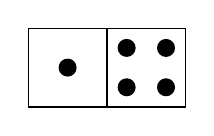
\begin{tikzpicture}
   [place/.style={circle,draw,fill=black,inner sep=0pt,thick,minimum size=2mm}]
   \def\rectanglepath{-- ++(1cm,0cm)-- ++(0cm,1cm)-- ++(-1cm,0cm) -- cycle}
   \draw (0,0) \rectanglepath;
   \draw (1,0) \rectanglepath;
   \node at (0.5,0.5) [place] {};
   \node at (1.25,0.75) [place] {};
   \node at (1.25,0.25) [place] {};
   \node at (1.75,0.75) [place] {};
   \node at (1.75,0.25) [place] {};
\end{tikzpicture}
\end{preview}
\end{document}


Además, recuerde que en el dominó cada lado de una pieza toma valores
entre 0 y 6 y que, por ejemplo, la pieza cuyos lados toman valores 1 y 4
es la misma que la pieza con valores 4 y 1.
                % :)
%\section{Lanzar dados}

Escriba un programa que muestre todas las combinaciones posibles al
momento de lanzar dos dados de 6 caras:


\chapter{Ruteos}
\section{Ojo con la indentación}

Sin usar el computador, rutee los siguientes tres programas e indique
cuál es la salida de cada uno de ellos.
Compruebe que sus respuestas son correctas
ejecutando los programas en el computador.

\begin{enumerate}
\item
\begin{lstlisting}
s = 0
t = 0
for i in range(3):
    for j in range(3):
        s = s + 1
        if i < j:
            t = t + 1
    print t
    print s
\end{lstlisting}

\item
\begin{lstlisting}
s = 0
t = 0
for i in range(3):
    for j in range(3):
        s = s + 1
    if i < j:
        t = t + 1
        print t
print s
\end{lstlisting}

\item
\begin{lstlisting}
s = 0
t = 0
for i in range(3):
    for j in range(3):
        s = s + 1
if i < j:
    t = t + 1
    print t
print s
\end{lstlisting}
\end{enumerate}


\section{Ruteos varios}

Solácese ruteando los siguientes programas.

\begin{enumerate}
\item
\begin{lstlisting}
j = 2
c = 1
p = True
while j > 0:
    j = j - c
    if p:
        c = c + 1
    p = not p
print j < 0 and p
\end{lstlisting}

\item
\begin{lstlisting}
a = 10
c = 1
x = 0
y = x + 1
z = y

while z <= y:
    z = z + c
    y = 2 * x + z
    if y < 4:
        y = y + 1
    x = x - 1

print x, y, z
\end{lstlisting}

\item
\begin{lstlisting}
a = 11
b = a / 3
c = a / 2
n = 0

while a == b + c:
    n += 1
    b += c
    c = b - c
    if n % 2 == 0:
        a = 2 * a - 3
    print 100 * b + c
\end{lstlisting}

\item
\begin{lstlisting}
a = True
b = '1'
c = 2
while b[-1] not in '378':
    a = 0 == len(b) % 2
    if a:
        c = c * 7
    b = b + str(c)
print c
\end{lstlisting}
\end{enumerate}


\chapter{Diseño de algoritmos}
\section{Dígitos}

Escriba un programa que determine la cantidad de dígitos en un número
entero ingresado por el usuario:
                      % :)
%\section{Dígito verificador}

Desarrolle un programa que calcule el dígito verificador de un rol
UTFSM.

Para calcular el dígito verificador, se deben realizar los siguiente
pasos:

\begin{enumerate}
\item
  Obtener el rol sin guión ni dígito verificador.
\item
  Invertir el número. (e.g: de 201012341 a 143210102).
\item
  Multiplicar los dígitos por la secuencia 2, 3, 4, 5, 6, 7, si es que
  se acaban los números, se debe comenzar denuevo, por ejemplo, con
  143210102:
\end{enumerate}

\[1\times2+ 4\times3+ 3\times4+ 2\times5+ 1\times6+ 0\times7+ 1\times2+ 0\times3+ 2\times4 = 52\]

\begin{enumerate}
\item
  Al resultado obtenido, es decir, 52, debemos sacarle el módulo 11, es
  decir:

  \begin{quote}
  52 \% 11 = 8
  \end{quote}
\item
  Con el resultado obtenido en el paso anterior, debemos restarlo de 11:

  \begin{quote}
  11 − 8 = 3
  \end{quote}
\item
  Finalmente, el dígito verificador será el obtenido en la resta:
  201012341-3.
\end{enumerate}

\section{Ecuación primer grado}

Escriba un programa que pida los coeficientes de una ecuación de primer
grado \(ax + b = 0\). y que entregue la solución.

Una ecuación de primer grado puede
tener solución única, tener infinitas soluciones o no tener soluciones.

\begin{lstlisting}[language=testcase]
Ingrese a: `0`
Ingrese b: `3`

Sin solucion
\end{lstlisting}

\begin{lstlisting}[language=testcase]
Ingrese a: `4`
Ingrese b: `2`

Solucion unica: -0.5
\end{lstlisting}

\begin{lstlisting}[language=testcase]
Ingrese a: `0`
Ingrese b: `0`

No hay solucion unica.
\end{lstlisting}
        % :)
\section{Caballo de ajedrez}

Un tablero de ajedrez es una grilla de \(8\times 8\) casillas. Cada celda puede
ser representada mediante las coordenadas de su fila y su columna,
numeradas desde 1 hasta 8.

\begin{figure}
  \centering
  \documentclass{minimal}
\usepackage[pdftex,active,tightpage]{preview}
\usepackage[utf8]{inputenc}
\usepackage{mathpazo}
\usepackage{tikz}
\usetikzlibrary{calc,arrows,decorations}
\PreviewEnvironment{tikzpicture}

\begin{document}
\tikzstyle{knight}=[draw, shape=circle, fill=white]
\tikzstyle{jump}=[->, thick]
\tikzstyle{odd}=[black!40!red]
\tikzstyle{even}=[black!60]
\begin{tikzpicture}[yscale=-1, scale=.9]
  \foreach\n in {1,...,8} {
    \node at (-.25, \n - .5) {\n};
    \node at (\n - .5, -.25) {\n};
  }
  \foreach\row in {0,2,4,6} {
    \foreach\col in {1,3,5,7} {
      \fill[odd]  (\row, \col)     rectangle ++(1, 1);
      \fill[even] (\row, \col - 1) rectangle ++(1, 1);
    }
  }
  \foreach\row in {1,3,5,7} {
    \foreach\col in {0,2,4,6} {
      \fill[odd]  (\row, \col) rectangle ++(1, 1);
      \fill[even] (\row, \col + 1) rectangle ++(1, 1);
    }
  }
  \draw[white] (0, 0) grid      ++(8, 8);
  \draw[thick] (0, 0) rectangle ++(8, 8);

  \def\row{2}
  \def\col{8}
  \node[knight] (c1) at (\col - .5, \row - .5) {C};
  \draw [jump, out=180, in= 90] (c1) to (\col - 2 - .5, \row - 1 - .5);
  \draw [jump, out=180, in=-90] (c1) to (\col - 2 - .5, \row + 1 - .5);
  \draw [jump, out= 90, in=  0] (c1) to (\col - 1 - .5, \row + 2 - .5);

  \def\row{3}
  \def\col{4}
  \node[knight] (c1) at (\col - .5, \row - .5) {C};
  \draw [jump, out=180, in= 90] (c1) to (\col - 2 - .5, \row - 1 - .5);
  \draw [jump, out=180, in=-90] (c1) to (\col - 2 - .5, \row + 1 - .5);
  \draw [jump, out=-90, in=  0] (c1) to (\col - 1 - .5, \row - 2 - .5);
  \draw [jump, out= 90, in=  0] (c1) to (\col - 1 - .5, \row + 2 - .5);
  \draw [jump, out=  0, in= 90] (c1) to (\col + 2 - .5, \row - 1 - .5);
  \draw [jump, out=  0, in=-90] (c1) to (\col + 2 - .5, \row + 1 - .5);
  \draw [jump, out=-90, in=180] (c1) to (\col + 1 - .5, \row - 2 - .5);
  \draw [jump, out= 90, in=180] (c1) to (\col + 1 - .5, \row + 2 - .5);

\end{tikzpicture}

\end{document}


  \caption{Ejemplos de los movimientos posibles del caballo de ajedrez.}
  \label{fig:caballo-ajedrez}
\end{figure}

El \href{http://es.wikipedia.org/wiki/Caballo\_(ajedrez)}{caballo} es
una pieza que se desplaza en forma de L: su movimiento consiste en
avanzar dos casillas en una dirección y luego una casilla en una
dirección perpendicular a la primera,
como se muestra en la figura~\ref{fig:caballo-ajedrez}.

Escriba un programa que reciba como entrada las coordenadas en que se
encuentra un caballo, y entregue como salida todas las casillas hacia
las cuales el caballo puede desplazarse.

Todas las coordenadas mostradas deben estar dentro del tablero.

Si la coordenada ingresada por el usuario es inválida, el programa debe
indicarlo.

\begin{lstlisting}[language=testcase]
Ingrese coordenadas del caballo.
Fila: `2`
Columna: `8`

El caballo puede saltar de 2 8 a:
1 6
3 6
4 7
\end{lstlisting}

\begin{lstlisting}[language=testcase]
Ingrese coordenadas del caballo.
Fila: `3`
Columna: `4`

El caballo puede saltar de 3 4 a:
1 3
1 5
2 2
2 6
4 2
4 6
5 3
5 5
\end{lstlisting}

\begin{lstlisting}[language=testcase]
Ingrese coordenadas del caballo.
Fila: `1`
Columna: `9`

Posicion invalida.
\end{lstlisting}

           % :)
\section{Media armónica}

La media armónica de una secuencia de `n` números reales `x\_1, x\_2,
ldots, x\_n` se define como:

\[H = \frac{n}{\frac{1}{x_1} + \frac{1}{x_2} + \frac{1}{x_3} + \ldots + \frac{1}{x_n}}\]

Desarrolle un programa que calcule la media armónica de una secuencia de
números.

El programa primero debe preguntar al usuario cuántos números ingresará.
A continuación, pedirá al usuario que ingrese cada uno de los `n`
números reales. Finalmente, el programa mostrará el resultado.
               % :)
\section{Números palíndromos}

Un número natural es un
\href{http://es.wikipedia.org/wiki/Pal\%C3\%ADndromo}{palíndromo} si se
lee igual de izquierda a derecha y de derecha a izquierda.

Por ejemplo, 14941 es un palíndromo, mientras que 81924 no lo es.

Escriba un programa que indique si el número ingresado es o no
palíndromo:

\begin{lstlisting}[language=testcase]
Ingrese un numero: `14941`
14941 es palindromo
\end{lstlisting}

\begin{lstlisting}[language=testcase]
Ingrese un numero: `81924`
81924 no es palindromo
\end{lstlisting}
         % :)
\section{Palabras palíndromas}

Así como hay \href{es-numero-palindromo.html}{números palíndromos},
también hay palabras palíndromas, que son las que no cambian al invertir
el orden de sus letras.

Por ejemplo, «reconocer», «Neuquén» y «acurruca» son palíndromos.

\begin{enumerate}[1.]
\item
  Escriba un programa que reciba como entrada una palabra e indique si
  es palíndromo o no. Para simplificar, suponga que la palabra no tiene
  acentos y todas sus letras son minúsculas:
\item
  Modifique su programa para que reconozca oraciones palíndromas. La
  dificultad radica en que hay que ignorar los espacios:
\end{enumerate}
         % :)
\section{Cachipún}

En cada ronda del juego del cachipún, los dos competidores deben elegir
entre jugar tijera, papel o piedra.

Las reglas para decidir quién gana la ronda son: tijera le gana a papel,
papel le gana a piedra, piedra le gana a tijera, y todas las demás
combinaciones son empates.

El ganador del juego es el primero que gane tres rondas.

Escriba un programa que pregunte a cada jugador cuál es su jugada,
muestre cuál es el marcador después de cada ronda, y termine cuando uno
de ellos haya ganado tres rondas. Los jugadores deben indicar su jugada
escri\-biendo \lstinline!tijera!, \lstinline!papel! o \lstinline!piedra!.

\begin{lstlisting}[language=testcase]
A: `tijera`
B: `papel`
1 - 0

A: `tijera`
B: `tijera`
1 - 0

A: `piedra`
B: `papel`
1 - 1

A: `piedra`
B: `tijera`
2 - 1

A: `papel`
B: `papel`
2 - 1

A: `papel `
B: `piedra`
3 - 1

A es el ganador
\end{lstlisting}
                     % :)
\section{Números primos}

El siguiente programa muestra la cantidad de números primos indicada por
el usuario:

En este programa, vemos que es posible declarar varias variables del
mismo tipo en una única sentencia (\lstinline!primos_por_mostrar!,
\lstinline!n! y \lstinline!d!).

También aprovechamos de presentar cómo se hacen los comentarios en C:
comienzan con \lstinline!/*! y terminan con \lstinline!*/!.

Escriba, compile y ejecute este programa.

\subsection{Sentencias de control: while, for e if}

Este programa muestra tres de las sentencias de control de C, que son
equivalentes a sus tocayos de Python: \lstinline!while!, \lstinline!for!
e \lstinline!if!.

El \lstinline!while! y el \lstinline!if! son sencillos. Hay que tener en
cuenta que la condición debe ir necesariamente entre paréntesis. El
contenido no se indica usando indentación, sino que encerrándolo entre
paréntesis de llave:

\begin{lstlisting}
while (condicion) {
    /* ... */
}

if (condicion) {
    /* ... */
}
\end{lstlisting}

(Aunque al compilador la indentación no le interesa, a los seres humanos
sí les ayuda a entender mejor el código, por lo que no indentar es una
pésima idea.)

Al igual que en Python, el \lstinline!if! puede ir seguido de un
\lstinline!else!. El \lstinline!elif! de Python no existe en C, pues es
legal escribir \lstinline!else if!.

El ciclo \lstinline!for! es un poco diferente. Entre los paréntesis
tiene tres partes separadas por punto y coma:

\begin{lstlisting}
for (inicializacion; condicion; actualizacion) {
    /* ... */
}
\end{lstlisting}

La inicialización se ejecuta una vez, antes de iniciar el ciclo. Aquí se
suele asignar un valor inicial a un contador.

La actualización es la parte donde se modifica el valor del contador al
final de cada iteración.

La condición es evaluada después de cada actualización, para decidir si
se continúa o no ejecutando el ciclo.

Algunos ejemplos de ciclos \lstinline!for! en C, junto con sus
equivalentes en Python:

\begin{lstlisting}
for (i = 0; i < N; ++i)       /* for i in range(N):         */
for (i = 5; i < 10; ++i)      /* for i in range(5, 10):     */
for (i = 2; i < 30; i += 2)   /* for i in range(2, 30, 2):  */
for (i = 40; i > 0; --i)      /* for i in range(40, 0, -1): */
for (i = 1; i <= N; ++i)      /* for i in range(1, N + 1):  */
\end{lstlisting}

Las sentencias \lstinline!break! y \lstinline!continue! de Python
también funcionan en C.

\subsection{Operadores de incremento y decremento}

La expresión \lstinline!n++! incrementa en uno el valor de
\lstinline!n!. Es decir, si \lstinline!n! tiene el valor 15, después de
hacer \lstinline!n++! tendrá el valor 16.

De manera similar, \lstinline!primos_por_mostrar--! reduce en uno el
valor de \lstinline!primos_por_mostrar!. Inicialmente esta variable
tiene el valor ingresado por el usuario, y luego va decreciendo hasta
llegar a cero. Cuando esto ocurre, el ciclo \lstinline!while! se
termina.

Ambos operadores pueden ir antes o después de la variable:

\begin{lstlisting}
n++;
++n;
\end{lstlisting}

Ambas modifican el valor de \lstinline!n! de la misma manera, pero
existe una diferencia sutil entre ambos que por ahora omitiremos.

\subsection{Valores lógicos}

En C no existe un tipo de datos para representar valores lógicos, como
el tipo \lstinline!bool! de Python. En C, \textbf{los valores lógicos
son enteros}. El valor cero es interpretado como falso, y cualquier otro
valor como verdadero.

Como ilustración, nuestro programa usa la variable \lstinline!es_primo!
para recordar si el número \lstinline!n! que se está analizando en cada
iteración es o no primo. Esta variable es entera, y su valor es cambiado
a cero apenas se encuentra un divisor.

Como los enteros pueden ser interpretados como valores lógicos, el ciclo
\lstinline!while! de nuestro programa también podría haber sido escrito
así:

\begin{lstlisting}
while (primos_por_mostrar) {
    /* ... */
}
\end{lstlisting}

ya que esto también haría que el ciclo terminara cuando la variable
llega a cero, porque en este caso sería interpretado como una condición
falsa. Haga la prueba, y convénzase de que funciona.

Los operadores lógicos en C son:

\begin{itemize}
\item
  \lstinline!&&! (y),
\item
  \lstinline!||! (o),
\item
  \lstinline"!" (negación).
\end{itemize}

Por ejemplo, si uno quisiera modificar el programa para que mostrara
sólo los números compuestos que terminan en 7, habría que cambiar la
condición del último \lstinline!if! por la siguiente:

\begin{lstlisting}
if (!es_primo && n % 10 == 7) {
    /* ... */
}
\end{lstlisting}

Los operadores \lstinline!==!, \lstinline"!=", \lstinline!<!,
\lstinline!>!, \lstinline!<=! y \lstinline!>=! funcionan de la misma
manera que en Python.

Uno de los errores más comunes en C es confundir el operador de igualdad
\lstinline!==! con la asignación \lstinline!=!. En C es legal poner una
asignación dentro de la condición de un \lstinline!if! o de un
\lstinline!while!, por lo que un programa como éste:

\begin{lstlisting}
if (x = 2) {
    /* ... */
}
\end{lstlisting}

compilará y se ejecutará sin errores, pero probablemente no hará lo que
nosotros esperamos: en vez de verificar que \lstinline!x! vale 2,
¡modificará \lstinline!x! para que lo valga!

\subsection{Ejercicios}

Modifique el programa de arriba para que, en vez de mostrar una cierta
cantidad de números primos, muestre todos los números primos menores que
\emph{m}.

A continuación, modifíquelo para que en lugar de mostrar sólo los
números primos los muestre todos, indicando para cada uno de ellos si es
primo o compuesto:
               % :)
\section{El mejor número}

Según Sheldon\footnote{\url{http://www.youtube.com/watch?v=Gg9kSn3NRVk}},
el mejor número es el 73.

73 es el 21er número primo. Su espejo, 37, es el 12mo número primo. 21
es el producto de multiplicar 7 por 3. En
\href{http://es.wikipedia.org/wiki/Sistema\_binario}{binario}, 73 es un
palíndromo: 1001001.

Escriba programas que le permitan responder las siguientes preguntas:
\begin{enumerate}
\item
  ¿Existen otros valores \(p\) que sean el \(n\)-ésimo primo,
  tales que \(\text{espejo}(p)\) es el \(\text{espejo}(n)\)-ésimo primo?
\item
  ¿Existen otros valores \(p\) que sean el \(n\)-ésimo primo, tales que \(n\)
  es el producto de los dígitos de \(p\)?
\item
  ¿Cuáles son los primeros diez números primos cuya representación
  binaria es un palíndromo?
\end{enumerate}
              % :)
\section{Adivinar el número}

Escriba un programa que «piense» un número entre 0 y 100, y entregue
pistas al usuario para que lo adivine.

El programa puede obtener un número al azar entre 0 y 100 de la
siguiente manera (¡haga la prueba!):

\begin{lstlisting}
>>> from random import randrange
>>> n = randrange(101)
>>> print n
72
\end{lstlisting}

El usuario debe ingresar su intento, y el programa debe decir si el
número pensado es mayor, menor, o el correcto:
\begin{lstlisting}[language=testcase]
Adivine el numero.
Intento 1: `32`
Es mayor que 32
Intento 2: `80`
Es menor que 80
Intento 3: `70`
Es mayor que 70
Intento 4: `72`
Correcto. Adivinaste en 4 intentos.
\end{lstlisting}

Una vez que complete ese ejercicio, es hora de invertir los roles: ahora
usted pensará un número y el computador lo adivinará.

Escriba un programa que intente adivinar el número pensado por el
usuario. Cada vez que el computador haga un intento, el usuario debe
ingresar \lstinline!<!, \lstinline!>! o \lstinline!=!, dependiendo si el
intento es menor, mayor o correcto.

La estrategia que debe seguir el programa es recordar siempre cuáles son
el menor y el mayor valor posibles, y siempre probar con el valor que
está en la mitad. Por ejemplo, si usted piensa el número 82, y no hace
trampa al jugar, la ejecución del programa se verá así:

\begin{lstlisting}[language=testcase]
Intento 1: 50
`>`
Intento 2: 75
`>`
Intento 3: 88
`<`
Intento 4: 81
`>`
Intento 5: 84
`<`
Intento 6: 82
`=`
Adivine en 6 intentos B-)
\end{lstlisting}

              % :)
%\section{Suma de tres cubos}

Es posible expresar 100 como la suma de tres cubos, cada uno de los
cuales puede ser negativo o positivo.

Sólo se conocen tres maneras de hacerlo. Una de ellas es la siguiente:

\[1870^{3} - 1797^{3} - 903^{3} = 100.\]

Desarrolle un programa que entregue las otras dos maneras.

\section{Números de Fibonacci}

Los
\href{http://es.wikipedia.org/wiki/N\%C3\%BAmeros\_de\_Fibonacci}{números
de Fibonacci} \(F_k\) son una sucesión de números naturales definidos de
la siguiente manera:
\begin{align*}
  F_0 &= 0, \\
  F_1 &= 1, \\
  F_k &= F_{k - 1} + F_{k - 2} \qquad\text{cuando } k\ge 2.
\end{align*}

En palabras simples, la sucesión de Fibonacci comienza con 0 y 1, y los
siguientes términos siempre son la suma de los dos anteriores.

\begin{table}
  \centering
  \begin{tabular}{l*{14}{r}}
    \toprule
    $n$   & 0 & 1 & 2 & 3 & 4 & 5 & 6 &  7 &  8 &  9 & 10 & 11 &  12 & \ldots{} \\
    \midrule
    $F_n$ & 0 & 1 & 1 & 2 & 3 & 5 & 8 & 13 & 21 & 34 & 55 & 89 & 144 & \ldots{} \\
    \bottomrule
  \end{tabular}
  \caption{Los primeros términos \(F_n\) de la sucesión de Fibonacci.}
  \label{tbl:fibonacci}
\end{table}

En la tabla~\ref{tbl:fibonacci} podemos ver los números de Fibonacci desde el
0-ésimo hasta el duodécimo.

\begin{enumerate}

  \item
    Escriba un programa que reciba como entrada un número entero \(n\),
    y entregue como salida el \(n\)-ésimo número de Fibonacci:

\begin{lstlisting}[language=testcase]
Ingrese n: `11`
F11 = 89
\end{lstlisting}

  \item
    Escriba un programa que reciba como entrada un número entero e indique
    si es o no un número de Fibonacci:

\begin{lstlisting}[language=testcase]
Ingrese un numero: `34`
34 es numero de Fibonacci
\end{lstlisting}

\begin{lstlisting}[language=testcase]
Ingrese un numero: `78`
78 no es numero de Fibonacci
\end{lstlisting}

  \item
    Escriba un programa que muestre los \(m\) primeros números de
    Fibonacci, donde \(m\) es un número ingresado por el usuario:

\begin{lstlisting}[language=testcase]
Ingrese m: `7`
Los 7 primeros numeros de Fibonacci son:
0 1 1 2 3 5 8
\end{lstlisting}

\end{enumerate}

%\section{Espiral}

\emph{Ejercicio sacado de Project Euler\footnotemark.}
\footnotetext{
  Publicado en \url{http://projecteuler.net/problem=28}
  bajo licencia Creative Commons BY-NC-SA 2.0.
}

La siguiente espiral de \(5 × 5\) se forma comenzando por el número 1, y
moviéndose a la derecha en el sentido de las agujas del reloj:

\begin{tabular}{*{5}{r}}
  \textbf{21} &         22  &         23  &         24  & \textbf{25} \\
          20  & \textbf{ 7} &          8  & \textbf{ 9} &         10  \\
          19  &          6  & \textbf{ 1} &          2  &         11  \\
          18  & \textbf{ 5} &          4  & \textbf{ 3} &         12  \\
  \textbf{17} &         16  &         15  &         14  & \textbf{13} \\
\end{tabular}

La suma de las diagonales de esta espiral es 101.

Escriba un programa que entregue la suma de las diagonales de una
espiral de \(1001 × 1001\) creada de la misma manera.

%\section{Suma de dígitos al cubo}

Entre todos los enteros mayores a 1 hay solamente cuatro que pueden ser
representados por la suma de los cubos de sus dígitos.

Uno de esos números es 153 pues:

\[1^3 + 5^3 + 3^3 = 1 + 125 + 27 = 153\]

Desarrolle un programa para poder determinar los otros tres números.

Tenga en cuenta que los números se encuentran entre 150 y 410.

%\section{Multiplicación rusa}

El método de
\href{http://mathworld.wolfram.com/RussianMultiplication.html}{multiplicación
rusa} consiste en multiplicar sucesivamente por 2 el multiplicando y
dividir por 2 el multiplicador hasta que el multiplicador tome el valor
1. Luego, se suman todos los multiplicandos correspondientes a los
multiplicadores impares.

Dicha suma es el producto de los dos números. La siguiente tabla muestra
el cálculo realizado para multiplicar 37 por 12, cuyo resultado final es
12 + 48 + 384 = 444.

\ctable[pos = H, center, botcap]{llll}
{% notes
}
{% rows
\FL
Multiplicador & Multiplicando & Multiplicador impar & Suma
\ML
37 & 12 & sí & 12
\\\noalign{\medskip}
18 & 24 & no & 
\\\noalign{\medskip}
9 & 48 & sí & 60
\\\noalign{\medskip}
4 & 96 & no & 
\\\noalign{\medskip}
2 & 192 & no & 
\\\noalign{\medskip}
1 & 384 & sí & 444
\LL
}

Desarrolle un programa que reciba como entrada el multiplicador y el
multiplicando, y entrege como resultado el producto de ambos, calculado
mediante el método de multiplicación rusa.

%\section{Números amistosos}

Un par de números \emph{m} y \emph{n} son llamados \textbf{amistosos} (o
se conocen como un \textbf{par amigable}), si la suma de todos los
divisores de \emph{m} (excluyendo a \emph{m}) es igual al número
\emph{n}, y la suma de todos los divisores del número \emph{n}
(excluyendo a \emph{n}) es igual a \emph{m} (con \emph{m} ≠ \emph{n}).

Por ejemplo, los números 220 y 284 son un par amigable porque los únicos
números que dividen de forma exacta 220 son 1, 2, 4, 5, 10, 11, 20, 22,
44, 55 y 110, y

\begin{quote}
1 + 2 + 4 + 5 + 10 + 11 + 20 + 22 + 44 + 55 + 110 = 284
\end{quote}

Por lo tanto, 220 es un número amistoso. Los únicos números que dividen
exactamente 284 son 1, 2, 4, 71 y 142 y

\begin{quote}
1 + 2 + 4 + 71 + 142 = 220
\end{quote}

Por lo tanto, 284 es un número amistoso.

Muchos pares de números amigables son conocidos; sin embargo, sólo uno
de los pares (220, 284) tiene valores menores que 1000. El siguiente par
está en el rango {[}1000, 1500{]}.

Desarrolle un programa que permita encontrar dicho par.

%\section{Método de Newton}

\emph{
  Ejercicio sacado de \emph{SICP}.\footnotemark.
}
\footnotetext{
  Harold Abelson, Gerald Jay Sussman y Julie Sussman.
  \emph{Structure and Interpretation of Computer Programs},
  2da edición.
  Publicado en \url{http://mitpress.mit.edu/sicp/}
  bajo licencia Creative Commons BY-SA 3.0.
  ¡Este libro es un clásico!
}

El método computacional más común para calcular raíces cuadradas
(y otras funciones también) es el
\href{http://es.wikipedia.org/wiki/M\%C3\%A9todo\_de\_Newton}{método de Newton}
de aproximaciones sucesivas. Cada vez que tenemos una estimación
\(y\) del valor de la raíz cuadrada de un número \(x\), podemos hacer una
pequeña manipulación para obtener una mejor aproximación (una más
cercana a la verdadera raíz cuadrada) promediando \(y\) con \(x/y\).

\begin{table}
  \centering
  \begin{tabular}{lll}
    \toprule
      Estimación \(y\) & Cuociente \(x/y\)     & Promedio \\
    \midrule
      \(1\)            & \(2/1      = 2\)      & \((2 + 1)          /2 = 1.5\)    \\
      \(1.5\)          & \(2/1.5    = 1.3333\) & \((1.3333 + 1.5 )  /2 = 1.4167\) \\
      \(1.4167\)       & \(2/1.4167 = 1.4118\) & \((1.4118 + 1.4167)/2 = 1.4142\) \\
      \(1.4142\)       & \ldots{}              & \ldots{} \\
    \bottomrule
  \end{tabular}
  \caption{Primeras iteraciones del método de Newton para aproximar la raíz cuadrada de 2
    usando la aproximación inicial 1.}
  \label{tbl:iteraciones-newton}
\end{table}

La tabla~\ref{tbl:iteraciones-newton} muestra cómo refinar paso a paso
la raíz cuadrada de dos a partir de la aproximación inicial \(\sqrt{2}\approx 1\).

Al continuar este proceso, obtenemos cada vez mejores estimaciones de la
raíz cuadrada.

El algoritmo debe detenerse cuando la estimación es «suficientemente
buena», que puede ser cualquier criterio bien definido.

\begin{enumerate}
\item
  Escriba un programa que reciba como entrada un número real \(x\) y
  calcule su raíz cuadrada usando el método de Newton. El algoritmo debe
  detenerse cuando el cuadrado de la raíz cuadrada estimada difiera de
  \(x\) en menos de 0,0001.

  (Este criterio de detención no es muy bueno).
\item
  Escriba un programa que reciba como entrada el número real \(x\) y un
  número entero indicando con cuántas cifras decimales de precisión se
  desea obtener su raíz cuadrada.

  El método de Newton debe detenerse cuando las cifras de precisión
  deseadas no cambien de una iteración a la siguiente.

  Por ejemplo, para calcular~\(\sqrt{2}\) con dos cifras de precisión,
  las estimaciones sucesivas son 1; 1,5; 1,416667 y 1,414216.
  El algoritmo debe detenerse en la cuarta iteración, pues en
  ella las dos primeras cifras decimales no cambiaron con respecto a la
  iteración anterior:

\begin{lstlisting}[language=testcase]
Ingrese x: `2`
Cifras decimales: `2`
La raiz es 1.4142156862745097
\end{lstlisting}

  (La cuarta aproximación es bastante cercana a la verdadera raíz
  1.4142135623730951).
\end{enumerate}

%\section{Triángulo de Pascal}

\begin{figure}
  \centering
  \documentclass[dvipsnames]{minimal}
\usepackage[pdftex,active,tightpage]{preview}
\usepackage{mathpazo}
\usepackage{tikz}
\usetikzlibrary{positioning,arrows}

\begin{document}
\begin{preview}
\begin{tikzpicture}[xscale=1.2, yscale=0.8]

  % Thanks to Paul Gaborit for this code.
  % http://www.texample.net/tikz/examples/pascals-triangle-and-sierpinski-triangle/

  % Pascal's triangle
  % row #0 => value is 1
  \node (p-0-0) at (0,0) {1};
  \foreach \row in {1,...,6} {
     % col #0 => value is 1
    \node (p-\row-0) at (-\row/2,-\row) {1};
    \pgfmathsetmacro{\value}{1};
    \foreach \col in {1,...,\row} {
      % iterative formula : val = precval * (row-col+1)/col
      % (+ 0.5 to bypass rounding errors)
      \pgfmathtruncatemacro{\value}{\value*((\row-\col+1)/\col)+0.5};
      \global\let\value=\value
      % position of each value
      \coordinate (pos) at (-\row/2+\col,-\row);
      \node (p-\row-\col) at (pos) {\value};
      % for arrows and plus sign
      \ifnum \col<\row
        \node[Red, above=0mm of p-\row-\col]{+};
        \pgfmathtruncatemacro{\prow}{\row-1}
        \pgfmathtruncatemacro{\pcol}{\col-1}
        \draw[Red, -latex'] (p-\prow-\pcol) -- (p-\row-\col);
        \draw[Red, -latex'] (p-\prow-\col) -- (p-\row-\col);
      \fi
    }
  }

\end{tikzpicture}
\end{preview}
\end{document}


  \label{fig:triangulo-pascal}
  \caption{Triángulo de Pascal}
\end{figure}

Desarrolle un programa que dibuje un
triángulo de Pascal, o sea, una disposición de números enteros tales que cada uno
sea la suma de los dos que están por encima de él,
tal como se ve en la figura~\ref{fig:triangulo-pascal}.

Un programa que genere las primeras cinco líneas
podría verse así:
\begin{lstlisting}[language=testcase]
1
1  1
1  2  1
1  3  3  1
1  4  6  4  1
1  5 10 10  5  1
\end{lstlisting}
o así:
\begin{lstlisting}[language=testcase]
          1
        1   1
      1   2   1
    1   3   3   1
  1   4   6   4   1
1   5  10  10   5   1
\end{lstlisting}
Usted, empero, debe generar las primeras veinte líneas.
Considere que en la línea 20 aparecen números de cinco dígitos.


%\section{Torre y alfil}

\emph{Este problema apareció en el certamen 1 del primer semestre de
2011.}

Un tablero de ajedrez es una grilla de ocho filas y ocho columnas,
numeradas de 1 a 8. Dos de las piezas del juego de ajedrez son el alfil
y la torre. El alfil se desplaza en diagonal, mientras que la torre se
desplaza horizontal o verticalmente. Una pieza puede ser capturada por
otra si está en una casilla a la cual la otra puede desplazarse:

\includegraphics{../../diagramas/torre-alfil.png}

Escriba un programa que reciba como entrada las posiciones en el tablero
de un alfil y de una torre, e indique cuál pieza captura a la otra:

Suponga que los datos ingresados son válidos. Su programa debe funcionar
para tableros de cualquier tamaño.

%\section{Rango}

\emph{Este problema apareció en el certamen 1 del primer semestre de
2011.}

En estadística descriptiva, se define el \emph{rango} de un conjunto de
datos reales como la diferencia entre el mayor y el menor de los datos.

Por ejemplo, si los datos son:

\begin{quote}
{[}5.96, 6.74, 7.43, 4.99, 7.20, 0.56, 2.80{]},
\end{quote}

entonces el rango es 7.43 − 0.56 = 6.87.

Escriba un programa que:

\begin{itemize}
\item
  pregunte al usuario cuántos datos serán ingresados,
\item
  pida al usuario ingresar los datos uno por uno, y
\item
  entregue como resultado el rango de los datos.
\end{itemize}

Suponga que todos los datos ingresados son válidos.

%\section{Valor actual neto}

\emph{Este problema apareció en el certamen 1 del primer semestre de
2011.}

En finanzas, el \emph{valor actual neto} es un indicador de cuán
rentable será un proyecto.

Se calcula sumando los flujos de dinero de cada mes divididos por `(1 +
r)\^{}n`, donde `n` es el número del mes y `r` es la tasa de descuento
mensual, y restando la inversión inicial.

Por ejemplo, en un proyecto en que la inversión inicial es \$900, los
flujos de dinero estimados para los primeros cuatro meses son \$550,
\$230, \$341 y \$190, y la tasa de descuento mensual es de 4\%, el valor
actual neto es:

\[\text{VAN} = -900 +
\frac{550}{(1 + 0.04)^1} +
\frac{230}{(1 + 0.04)^2} +
\frac{341}{(1 + 0.04)^3} +
\frac{190}{(1 + 0.04)^4}.\]

Si el VAN da negativo, entonces no es conveniente comenzar el proyecto.

Escriba un programa que pida al usuario ingresar la inversión inicial y
el porcentaje de tasa de descuento. A continuación, debe preguntar el
flujo de dinero estimado para cada mes y mostrar cuál es la parte entera
del VAN hasta ese momento.

El programa debe terminar apenas el VAN comience a dar positivo.

Suponga que todos los datos ingresados son válidos.

%\section{Reglamento de evaluaciones}

\emph{Este problema apareció en el certamen 1 del segundo semestre de
2011 en el campus Vitacura.}

La Universidad Tropical Filomena Santa Marta ha instaurado un nuevo
reglamento de evaluaciones. Todas las asignaturas deben tener tres
certámenes y un examen. Las notas van entre 0 y 10, con un decimal.

Después de los tres certámenes, los alumnos con promedio menor que 3
reprueban y los con promedio mayor o igual que 7 aprueban. El resto va
al examen, en el que deben sacarse por lo menos un 5 para aprobar.

Además, para reducir el trabajo de los profesores, se decidió que los
alumnos que se sacan menos de un 2 en los dos primeros certámenes están
automáticamente reprobados. A su vez, los que obtienen más de un 9 en
los dos primeros certámenes están automáticamente aprobados. En ambos
casos, no deben rendir el tercer certamen.

Escriba un programa que pregunte a un estudiante las notas de las
evaluaciones que rindió, y le diga si está aprobado o reprobado.

%\section{Votaciones de la CONFECH}

\emph{Este problema apareció en el certamen 1 del segundo semestre de
2011 en el campus Vitacura.}

La CONFECH, en su afán de agilizar el proceso de recuento de las
votaciones, le ha encargado el desarrollo de un programa de registro de
votación por universidades.

Primero, el programa debe solicitar al usuario ingresar la cantidad de
universidades que participan en el proceso.

Luego, para cada una de las universidades, el usuario debe ingresar el
nombre de la universidad y los votos de sus alumnos, que pueden ser:
\emph{aceptar} (\lstinline!A!), \emph{rechazar} (\lstinline!R!),
\emph{nulo} (\lstinline!N!) o \emph{blanco} (\lstinline!B!). El término
de la votación se indica ingresando una \lstinline!X!, tras lo cual se
debe mostrar los totales de votos de la universidad, con el formato que
se muestra en el ejemplo.

Finalmente, el programa debe mostrar el resultado de la votación,
indicando la cantidad de universidades que aceptan, que rechazan y en
las que hubo empate entre estas dos opciones.

%\section{Promoción con descuento}

\emph{Este problema apareció en el certamen 1 del segundo semestre de
2011 en el campus Vitacura.}

El supermercado Pitón Market ha lanzado una promoción para todos sus
clientes que posean la tarjeta Raw Input. La promoción consiste en
aplicar un descuento por cada \emph{n} productos que pasan por caja.

El primer descuento es de 20\%, y se aplica sobre los primeros \emph{n}
productos ingresados. Luego, cada descuento es la mitad del anterior, y
es aplicado sobre los siguientes \emph{n} productos.

Por ejemplo, si \emph{n} = 3 y la compra es de 11 productos, entonces
los tres primeros tienen 20\% de descuento, los tres siguientes 10\%,
los tres siguientes 5\%, y los dos últimos no tienen descuento.

Escriba un programa que pida al usuario ingresar \emph{n} y la cantidad
de productos, y luego los precios de cada producto. Al final, el
programa debe entregar el precio total, el descuento total y el precio
final después de aplicar el descuento.

Si al aplicar el descuento el precio queda con decimales, redondee el
valor hacia abajo.

%\section{Alzas del dólar}

\emph{Este problema apareció en el certamen recuperativo 1 del segundo
semestre de 2011 en el campus Vitacura.}

Un analista financiero lleva un registro del precio del dólar día a día,
y desea saber cuál fue la mayor de las alzas en el precio diario a lo
largo de ese período.

Escriba un programa que pida al usuario ingresar el número \emph{n} de
días, y luego el precio del dólar para cada uno de los \emph{n} días.

El programa debe entregar como salida cuál fue la mayor de las alzas de
un día para el otro.

Si en ningún día el precio subió, la salida debe decir:
\lstinline!No hubo alzas!.

%\section{Máquina de alimentos}

\emph{Este problema apareció en el certamen recuperativo 1 del segundo
semestre de 2011 en el campus Vitacura.}

Una máquina de alimentos tiene productos de tres tipos, \lstinline!A!,
\lstinline!B! y \lstinline!C!, que valen respectivamente \$270, \$340 y
\$390. La máquina acepta y da de vuelto monedas de \$10, \$50 y \$100.

Escriba un programa que pida al usuario elegir el producto y luego le
pida ingresar las monedas hasta alcanzar el monto a pagar. Si el monto
ingresado es mayor que el precio del producto, el programa debe entregar
las monedas de vuelto, una por una.

%\section{Intersección de circunferencias}

\emph{Este problema apareció en el certamen recuperativo 1 del segundo
semestre de 2011 en el campus Vitacura.}

Una circunferencia en el plano está definida por tres valores: las
coordenadas (\emph{x}, \emph{y}) de su centro, y su radio \emph{r}.

Escriba un programa que determine si dos circunferencias se intersectan
o no.

\includegraphics{../../diagramas/circunferencias-cert.png}

